\documentclass{article}

% if you need to pass options to natbib, use, e.g.:
%     \PassOptionsToPackage{numbers, compress}{natbib}
% before loading neurips_2021

% ready for submission
\usepackage[final]{neurips_2021}

% to compile a preprint version, e.g., for submission to arXiv, add add the
% [preprint] option:
%     \usepackage[preprint]{neurips_2021}

% to compile a camera-ready version, add the [final] option, e.g.:
%     \usepackage[final]{neurips_2021}

% to avoid loading the natbib package, add option nonatbib:
%    \usepackage[nonatbib]{neurips_2021}

\usepackage[utf8]{inputenc} % allow utf-8 input
\usepackage[T1]{fontenc}    % use 8-bit T1 fonts
\usepackage{hyperref}       % hyperlinks
\usepackage{url}            % simple URL typesetting
\usepackage{booktabs}       % professional-quality tables
\usepackage{amsfonts}       % blackboard math symbols
\usepackage{nicefrac}       % compact symbols for 1/2, etc.
\usepackage{microtype}      % microtypography
\usepackage{xcolor}         % colors
\usepackage{amsmath}
\usepackage{verbatim}
\usepackage[mathscr]{euscript}
\usepackage{graphicx}

\title{Machine Learning, 2024 Spring\\Assignment 6}
% The \author macro works with any number of authors. There are two commands
% used to separate the names and addresses of multiple authors: \And and \AND.
%
% Using \And between authors leaves it to LaTeX to determine where to break the
% lines. Using \AND forces a line break at that point. So, if LaTeX puts 3 of 4
% authors names on the first line, and the last on the second line, try using
% \AND instead of \And before the third author name.



\usepackage{listings}
\lstset{%
	alsolanguage=Java,
	%alsolanguage=[ANSI]C,      %可以添加很多个alsolanguage,如alsolanguage=matlab,alsolanguage=VHDL等
	alsolanguage= matlab,
	alsolanguage= XML,
	tabsize=4, %
	frame=shadowbox, %把代码用带有阴影的框圈起来
	commentstyle=\color{red!50!green!50!blue!50},%浅灰色的注释
	rulesepcolor=\color{red!20!green!20!blue!20},%代码块边框为淡青色
	keywordstyle=\color{blue!90}\bfseries, %代码关键字的颜色为蓝色,粗体
	showstringspaces=false,%不显示代码字符串中间的空格标记
	stringstyle=\ttfamily, % 代码字符串的特殊格式
	keepspaces=true, %
	breakindent=22pt, %
	numbers=left,%左侧显示行号 往左靠,还可以为right,或none,即不加行号
	stepnumber=1,%若设置为2,则显示行号为1,3,5,即stepnumber为公差,默认stepnumber=1
	%numberstyle=\tiny, %行号字体用小号
	numberstyle={\color[RGB]{0,192,192}\tiny} ,%设置行号的大小,大小有tiny,scriptsize,footnotesize,small,normalsize,large等
	numbersep=8pt,  %设置行号与代码的距离,默认是5pt
	basicstyle=\footnotesize, % 这句设置代码的大小
	showspaces=false, %
	flexiblecolumns=true, %
	breaklines=true, %对过长的代码自动换行
	breakautoindent=true,%
	breakindent=4em, %
	escapebegin=\begin{CJK*}{GBK}{hei},escapeend=\end{CJK*},
	aboveskip=1em, %代码块边框
	tabsize=2,
	showstringspaces=false, %不显示字符串中的空格
	backgroundcolor=\color[RGB]{245,245,244},   %代码背景色
	%backgroundcolor=\color[rgb]{0.91,0.91,0.91}    %添加背景色
	escapeinside=``,  %在``里显示中文
	%% added by http://bbs.ctex.org/viewthread.php?tid=53451
	fontadjust,
	captionpos=t,
	framextopmargin=1pt,framexbottommargin=1pt,abovecaptionskip=-3pt,belowcaptionskip=3pt,
	xleftmargin=2em,xrightmargin=2em, % 设定listing左右的空白
	% 设定中文冲突,断行,列模式,数学环境输入,listing数字的样式
	extendedchars=false,columns=flexible,mathescape=true
	% numbersep=-1em
}


\begin{document}
\author{
    Name: \textbf{Zhou Shouchen} \\\\
	Student ID: 2021533042
}
\maketitle

\begin{abstract}

\end{abstract}
\newpage

\textcolor{blue}{Problem 1}

Which of the following are possible growth functions $m_{\mathcal{H}}(N)$ for some hypothesis set:
$$
1+N ; 1+N+\dfrac{N(N-1)}{2} ; 2^N ; 2^{\lfloor\sqrt{N}\rfloor} ; 2^{\lfloor \frac{N}{2} \rfloor} ; 1+N+\dfrac{N(N-1)(N-2)}{6}
$$

\textcolor{blue}{Solution}\\
\begin{itemize}
    \item[1. ] $1+N$:\\
    Since $1+1=2^1$, and $1+2<2^2$, so $k=2$ is the breakpoint.
    $$\sum_{i=0}^{k-1} \binom{N}{i} = \sum_{i=0}^{1} \binom{N}{i} = 1+N$$
    Since $$m_{\mathcal{H}}(N)=1+N\leq \sum_{i=0}^{k-1} \binom{N}{i}$$
    So $m_{\mathcal{H}}(N)=1+N$ is a possible growth function.
    
    \item[2. ]  $1+N+\dfrac{N(N-1)}{2}$:\\
    Since $1+2+\dfrac{2*1}{2}=2^2$, and $1+3+\dfrac{3*2}{2}<2^3$, so $k=3$ is the breakpoint.
    $$\sum_{i=0}^{k-1} \binom{N}{i} = \sum_{i=0}^{2} \binom{N}{i} = 1+N+\dfrac{N(N-1)}{2}$$
    So $$m_{\mathcal{H}}(N)=1+N+\dfrac{N(N-1)}{2}\leq \sum_{i=0}^{k-1} \binom{N}{i}$$
    So $m_{\mathcal{H}}(N)=1+N+\dfrac{N(N-1)}{2}$ is a possible growth function.
    
    \item[3. ] $2^N$:\\
    $\forall k=1,2,\cdots,N$, we have
    $$m_{\mathcal{H}}(N)=2^N$$
    So the breakpoint is $k=\infty$.
    $$\sum_{i=0}^{k-1} \binom{N}{i} = 2^N$$
    So $$m_{\mathcal{H}}(N)=2^N\leq \sum_{i=0}^{k-1} \binom{N}{i}$$
    So $m_{\mathcal{H}}(N)=2^N$ is a possible growth function.
    
    \item[4.] $2^{\lfloor\sqrt{N}\rfloor}$:\\
    Since $2^{\lfloor\sqrt{1}\rfloor}=2^1$ and $2^{\lfloor\sqrt{2}\rfloor}<2^2$, so $k=2$ is the breakpoint.
    $$\sum_{i=0}^{k-1} \binom{N}{i} = \sum_{i=0}^{1} \binom{N}{i} = 1+N$$
    But $m_{\mathcal{H}}(N)=2^{\lfloor\sqrt{N}\rfloor}$ is close to a exponential function, and the $1+N$ is polynormial function, so it must has a $N$, such as $N=25$:
    $$m_{\mathcal{H}}(N)=32>1+N=26$$
    So $m_{\mathcal{H}}(N)=2^{\lfloor\sqrt{N}\rfloor}$ is not a possible growth function.

    \item[5.] $2^{\lfloor \frac{N}{2} \rfloor}$:\\
    Since $2^{\lfloor \frac{0}{2}\rfloor}=2^0$ and $2^{\lfloor \frac{1}{2}\rfloor}=1<2^1$, so $k=1$ is the breakpoint.
    $$\sum_{i=0}^{k-1} \binom{N}{i} = \sum_{i=0}^{0} \binom{N}{i} = 1$$
    But $m_{\mathcal{H}}(N)=2^{\lfloor\frac{N}{2}\rfloor}$ is an increasing function, and the $1$ is a constant function, so $\forall N\geq 2$
    $$m_{\mathcal{H}}(N)=2^{\lfloor \frac{N}{2}\rfloor}>1$$
    So $m_{\mathcal{H}}(N)=2^{\lfloor \frac{N}{2}\rfloor}$ is not a possible growth function.
    
    \item[6.] $1+N+\dfrac{N(N-1)(N-2)}{6}$:\\
    Since $1+1+\dfrac{1(1-1)(1-2)}{6}=2^1$ and $1+2+\dfrac{2(2-1)(2-2)}{6}=3<2^2$, so $k=2$ is the breakpoint.
    $$\sum_{i=0}^{k-1} \binom{N}{i} = \sum_{i=2}^{0} \binom{N}{i} = 1+N$$
    But when $\dfrac{N(N-1)(N-2)}{6}\neq 0$, i.e. $N\geq 3$, we have
    $$m_{\mathcal{H}}(N)=1+N+\dfrac{N(N-1)(N-2)}{6}>1+N$$
    So $m_{\mathcal{H}}(N)=1+N+\dfrac{N(N-1)(N-2)}{6}$ is not a possible growth function.
    
\end{itemize}
So above all, the possible growth functions $m_{\mathcal{H}}(N)$ are 
$$1+N ; 1+N+\dfrac{N(N-1)}{2}; 2^N $$
And the followings are not possible growth functions.
$$ 2^{\lfloor\sqrt{N}\rfloor} ; 2^{\lfloor \frac{N}{2} \rfloor}; 1+N+\dfrac{N(N-1)(N-2)}{6} $$

\newpage
\textcolor{blue}{Problem 2}

For an $\mathcal{H}$ with $d_{\mathrm{vc}}=10$, what sample size do you need (as prescribed by the generalization bound) to have a $95 \%$ confidence that your generalization error is at most 0.05 ?

\textcolor{blue}{Solution}\\








\newpage
\textcolor{blue}{Problem 3}
According to the iterative format provided as follow:
\begin{itemize}
    \item Use the SUV dataset to implement (using Python or MATLAB) the Gradient Descent method to find the optimal model for logistic regression.
    \item What is your test error? What are the sizes of the training set and test set, respectively?
    \item What is your learning rate? How was it chosen? How many steps were iterated in total?
    \item Present the results of the last 10 steps produced by your algorithm, including the loss, learning rate, the L2 norm of the gradient, and the number of function evaluations and gradient evaluations.
\end{itemize}
\begin{figure}[htbp]
\centerline{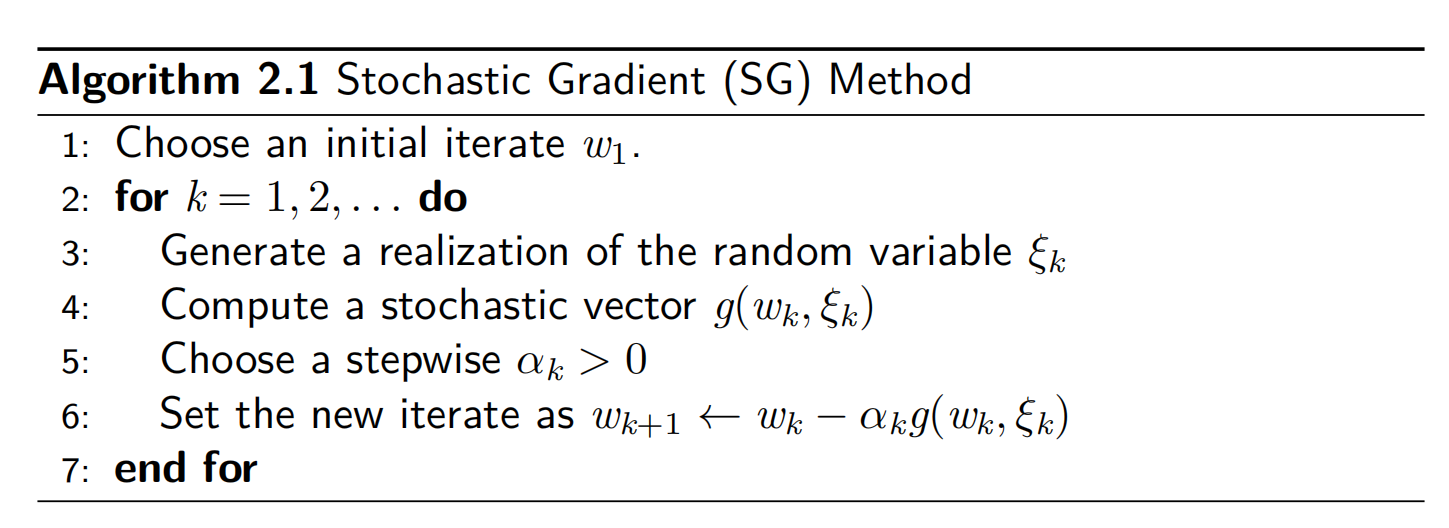
\includegraphics[width=\textwidth]{../image/alg.png}}
\href
  {https://www.cs.toronto.edu/~mhsadi/code-repository/MachineLearningNotebooks/3-SUVDataset.html}
  {Dataset reference and description}
  \\
\href
{https://www.kaggle.com/datasets/iamaniket/suv-data?resource=download}
  {Dataset and download}

\end{figure}

\textcolor{blue}{Solution}

0. Data preperation\\
After checking the SUV dataset, we could find that each buyer's information has a unique `User ID', so we can just drop the `User ID' column.\\
To use the `Gender' information, we map `Male' into $1$, and `Female' into $0$.\\
If we use exponential function during the logistic regression, it may have too big values with large `Age' and `EstimatedSalary', so we can seperate the `Age' and `EstimatedSalary' into different intervals.
And use an one-hot vector to represent the which range the `Age' and `EstimatedSalary' belongs to. And the modified encoding for `Age' and `Estimated salary' are as followed in Figure \ref{fig:age} and Figure \ref{fig:salary}.
The catagoies of `Age' and `EstimatedSalary' are chosen by the distribution graph of the original data, and each catagory is represented by a one-hot vector.\\

\begin{figure}[htbp]
  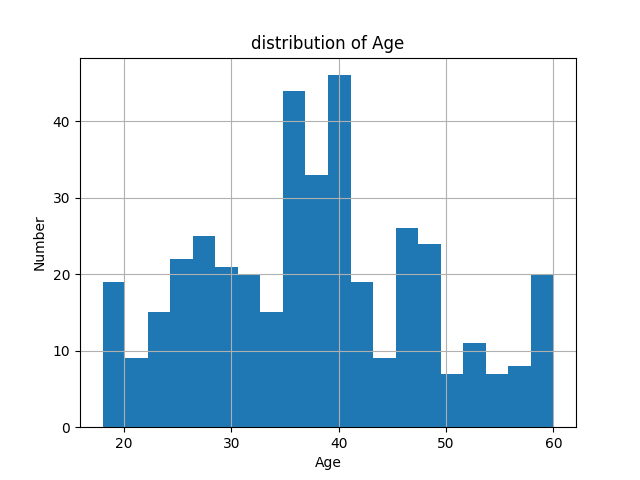
\includegraphics[width=0.5\textwidth]{../image/age_distribution.png}
  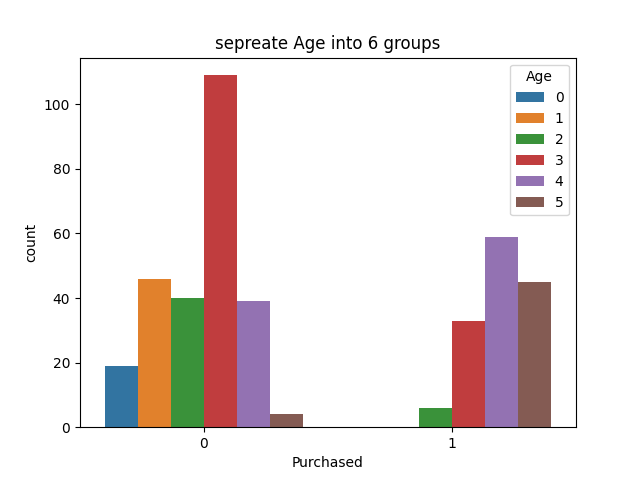
\includegraphics[width=0.5\textwidth]{../image/seperated_age.png}
  \caption{Analysis of Age}  
\label{fig:age}
\end{figure}

\begin{figure}[htbp]
  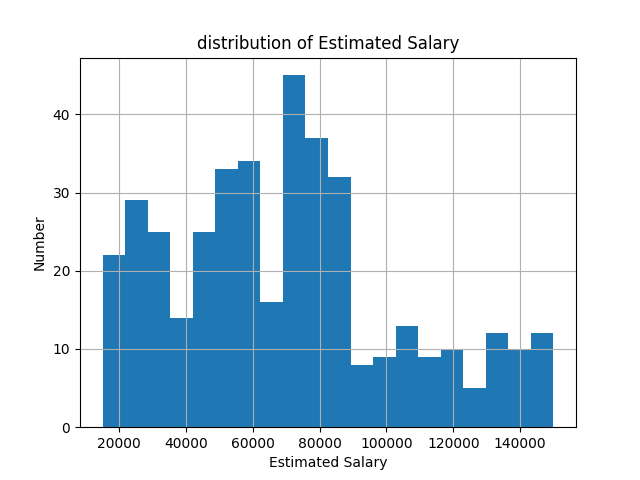
\includegraphics[width=0.5\textwidth]{../image/salary_distribution.png}
  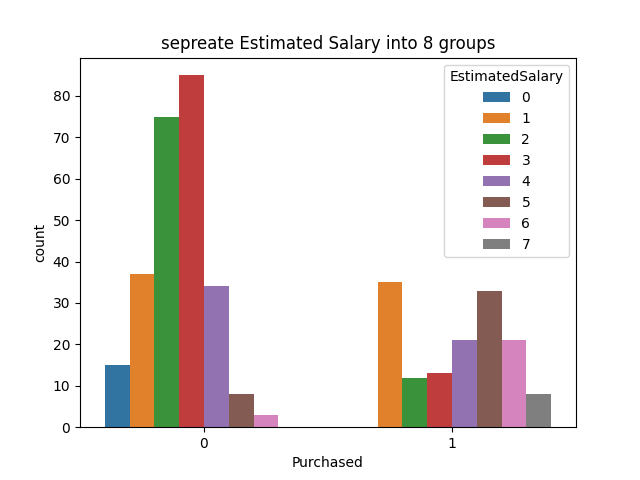
\includegraphics[width=0.5\textwidth]{../image/seperated_salary.png}
  \caption{Analysis of Estimated Salary}  
\label{fig:salary}
\end{figure}

To suit better for logistic regression, the `Purchased' column is also modified into `$-1$' for unpurchased and `$1$' for purchased.\\
At last, a bias term `$1$ is add for each input fetures. 
And before sending the data into the logistic regression, the input features are normalized.\\

Then the `Gender', `Age', `EstimatedSalary' can be used as the input features, and the `Purchased' can be used as the output label.\\
So this is a binary classification problem.\\
And we can use the logistic regression to solve this problem.\\

1. Since we are applying the logistic regression, so the testing error is:
$$E(\mathbf{w}) = \dfrac{1}{N}\sum_{i=1}^{N}\log (1+e^{-y_n\mathbf{w}^T\mathbf{x}_n})$$
which have been proved in Problem 1. And $N$ is the size of the testing set's size. $y_n$ are the labels of
testing set, $\mathbf{x}_n$ are the input data for the testing set.\\
The variation curve for the testing error is shown in Figure \ref{fig:testing}.\\

And the size of training set is $70$ persent, which is totally $280$ samples. And the testing set is $30$ persent, which is totally $120$ samples.\\
And before seperating the data, we random shuffled the total $400$ data with a fixed seed in order to make sure the randomness, but could be stable reproduction.\\

2. We have known that the gradient of logistic regression from Problem 1 is:
$$\nabla E_{\text {in }}(\mathbf{w}) = \dfrac{1}{N}\sum_{i=1}^{N}-y_n\mathbf{x}_n\theta(-y_n\mathbf{w}^T\mathbf{x}_n)$$
$\nabla E_{\text {in }}(\mathbf{w}),y_n,\mathbf{x}_n$ are set for the training set.\\
To set the learning rate getting smaller as the training iterations go on, we can set the learning rate as:
$$\eta_t = \eta\cdot \|\nabla E_{\text{in}}(\mathbf{w})\|$$
where $\eta=0.2$ is the initial learning rate, and $\|\nabla E_{\text{in}}(\mathbf{w})\|$ is the norm of the gradient.\\
And the total iterated steps is set to be $5000$ iterataions.\\ 

3. The results of the last 10 steps are shown in Figure \ref{fig:info}.\\
We could see that the training loss, the $L_2$ norm of the gradient $\|\nabla E_{\text{in}}(\mathbf{w})\|$ are dropping, but quite slow, which is close to get converage.\\
And the number of the gradient evaluations is once per iterataion, used for updating the $\mathbf{w}$.\\
And the number of the gradient evaluations is twice per iterataion, used for calculating the loss for both training set and the testing set.\\

\begin{figure}[htbp]
  \centerline{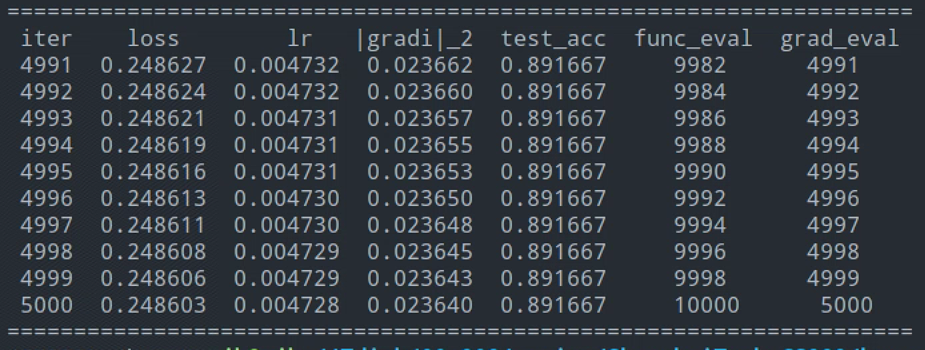
\includegraphics[width=\textwidth]{../image/info.png}}
  \caption{The last 10 steps' output} 
  \label{fig:info} 
\end{figure}

4. Analysis:\\
Figure \ref{fig:testing} are the testing accuracy and testing loss. From the 
testing loss, we could find that the model somehow overfitted on the training data, as the 
testing loss gradually becomes higher as the iterataions grow. But the testing accuracy was not effected so much,
it might because the dataset is small, and the data distribution are regular, so overfitting on the training set did not make testing accuracy got worse.\\

Figure \ref{fig:training} are the gradient's $L_2$ norm $\|\nabla E_{\text{in}}(\mathbf{w})\|$, the learning rate $\eta_t = \eta\cdot \|\nabla E_{\text{in}}(\mathbf{w})\|$, and the training loss.\\
The learning rate is obviously to have the same trend with the $\|\nabla E_{\text{in}}(\mathbf{w})\|$ as they have the proportional relationship. The training loss also has the 
quite same trend with them. Decreasing rapidly at first, and getting much slower as getting converage.\\

5. The code and the method to run the code are all in the folder `code'.

\begin{figure}[htbp]
  \centerline{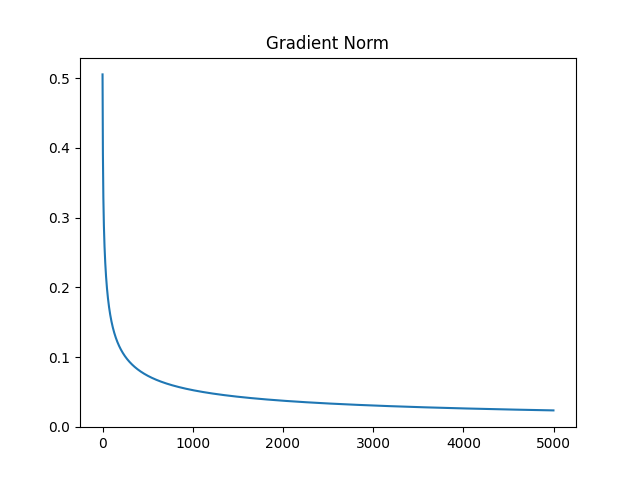
\includegraphics[width=0.7\textwidth]{../image/grad_norm.png}}
  \centerline{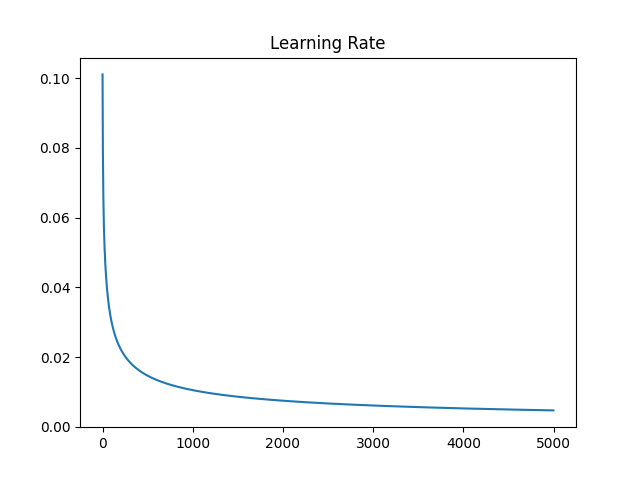
\includegraphics[width=0.7\textwidth]{../image/learning_rate.png}}
  \centerline{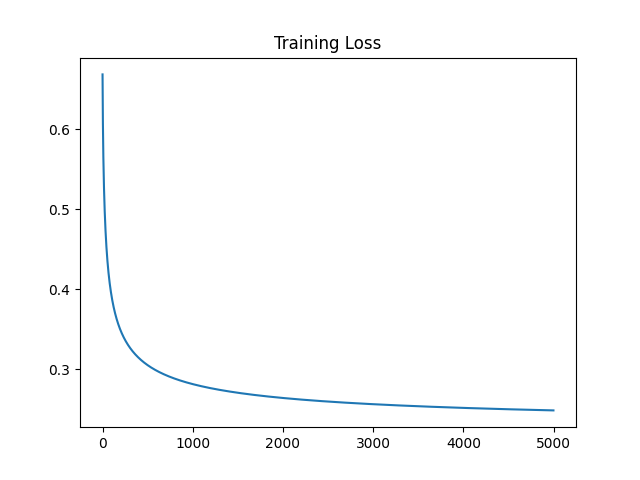
\includegraphics[width=0.7\textwidth]{../image/training_loss.png}}
  \caption{The training information}
  \label{fig:training}
\end{figure}

\begin{figure}[htbp]
  \centerline{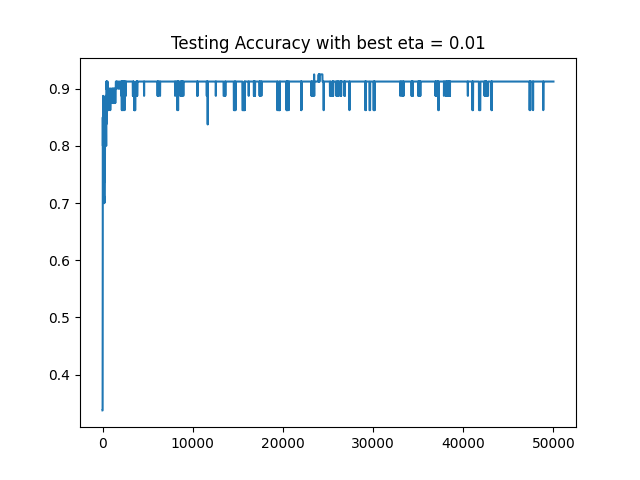
\includegraphics[width=\textwidth]{../image/testing_acc.png}}
  \centerline{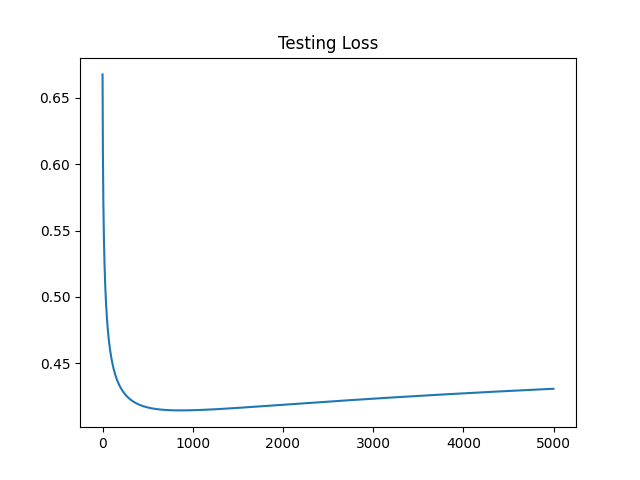
\includegraphics[width=\textwidth]{../image/testing_loss.png}}
  \caption{The testing information}
  \label{fig:testing}
\end{figure}

\end{document}